% LITERATURE REVIEW CHAPTER
\chapter{Literature Review}\label{ch:literaturereview}
This section aims to review previous literature of prediction models in the esports industry that was previously explored during Chapter~\ref{ch:introduction}.
These literatures will help create a better working understanding of how to properly model, extract and gain knowledge from the datasets.
It will cover papers from traditional sports where prediction models are widespread and lesser researched esports models, to research on the betting industry with its new relation to esports.
These studies will then be contextualised to form a set of research questions and aims, that will be answered through this paper.

\section{Predictive Analytics in Traditional Sports}\label{sec:TradSports}
In the mid to late 2000s the use of prediction modelling exploded academically, being applied to a multitude of fields from biology and medicine to political sciences or sports.
This academic surge of interest caused thousands of studies all using various forms of predictive modelling.
Not only did this evolve many practises across these fields, but it also helped develop the techniques of predictive modelling today.
This is section we will explore literature related to how predictive analytics are used in sports, and how insights can be gained from this type of modelling.
\citet{sarlis2020sports} studied the impact of how various basketball related performance evaluation metrics can be used to identify dominant attributes that will help predict candidates for the Most Valuable Player (MVP) award, as well as Defender of the Year in the National Basketball Association.
They concluded that using their Propagation Neural Networks with 8 years of training data, that their model was able to accurately predict the MVP of the season with 100\% accuracy, and could also predict the Defender of the Year.
Similar studies have been performed with football such as~\citet{pantzalis2020sports}, where they analysed 4 top football leagues in Europe and predicted the final standings with up to 70\% accuracy.
\citet{scelles2021peculiar} shows us that transferring this level of analysis from a traditional sports team to an esports team is highly supported, with claims that `esports\ldots~could provide some insights about the future development of sport`.
This suggests that prediction modelling is likely to work when used to predict both player performances, whilst potentially being able to predict standing of esports leagues globally. \\

\citet{wilkens2021sports} analysed professional tennis matches over the last decade, using player, match and betting data to produce an ensemble machine learning model to investigate how the informational content of these data points in relation to how they can help predict match outcomes.
They used their findings to evaluate whether bettors were able to achieve consistently positive returns.
Prediction accuracy was found to reach about 70\% with a complex model filled with all data previously mentioned, whilst a simpler baseline model using current world rankings was able to determine the result 65\% of the time.
Despite these results, they found potential returns of 10\% from a long-term betting strategy, however the volatility, total liquidity required and model risk makes the sentiment behind the model questionable at best.
A similar model is likely to translate well over to League of Legends, using potential features such as current league standings as a strong predictor variable as well as the historic match data that has already been collected. \\

\citet{thabtah2019nba} proposed a new machine learning framework that would help predict results in the Nation Basketball Association, and discover the most influential features that affect the outcome of NBA games.
Some models used throughout include Naïve Bayes, neural networks, and decision trees.
They concluded that there were five key performance metrics that were the most influential to any game played in the NBA\@.
Using these features they were able to achieve a prediction accuracy of up to 83\% using the Logistic Model Tree method. \\

These studies largely suggest that using predictive analytics for both player performance predictions, and team-wide predictions in traditional sports is highly successful, with studies concluding that they are able to predict match outcomes, league standings and league MVP votes consistently.
The majority of these studies also concluded that using either a classifier such as Random Forest and Gradient Boosting or Logistic Regression techniques were often optimal for maximising accuracy and AUC\@.
\citet{scelles2021peculiar} proposed a relationship between traditional sports and esports that suggests that similar predictive analytics techniques would have large crossover, and understanding this potential is fundamental in forming a basis for the value of the work in the esports field.

\section{Predictive Analytics in Esports}\label{sec:PredictiveAnalyticsinEsports}
\subsection{Match Outcome Prediction}\label{subsec:Match Outcome Prediction}
The work of predictive modelling in esports only started in the mid 2010s, with one of the original papers by~\citet{lin2016league} exploring match outcomes in League of Legends.
This work focused on the relationship between the potential feature-sets that a game such as League of Legends can create, and how they impact the predicted match outcome both pre-game and in-game.
The data was collected using the Riot API from matches with average ranked players, with the in-game data being extracted from the statistics published at the end of a match.
It becomes apparent that the data used in this initial study appears to be highly correlated with the match result, and this is reflected by the 95\% success rate on prediction using in-game data.
\citet{yang2016real} also investigated the match outcomes in another esports MOBA game, DOTA 2.
They considered pre-match features from individual players' historical performance data, as well as real-time data obtained during the match progression.
The effectiveness of the pre-match features seemed to be highly variable, with outcome prediction probabilities quoted at up to 71.49\%, and a model of combined pre-match and in-match data reaching up to 93.73\% accuracy at the 40th minute.
Interestingly, for the initial 15 minutes, the prediction accuracy for the real-time model is below that of the pre-match prediction values, potentially suggesting that the pre-match prediction accuracy could be inflated due to issues of interactions between features. \\

\citet{ravari2017predicting} once again considered match outcomes, but this is based upon First-Person Shooter game, Destiny.
Classification models were created based on the different game modes available, with a model based on specific game modes and a combined model.
They obtained results that highly favour models built upon data from specific game modes, concluding that the behavioural difference seen in players depending on the game mode is the main attributing factor.
These models were built upon the Random Forest algorithm and the Gradient Boosting classifier. \\

Two studies built upon the previous research just two years later.
\citet{silva2018continuous} introduces the use of \ac{RNN} to predict esports matches through time intervals between the 0 and 25 minute mark, and uses data from matches between 2015 to early 2018.
They concluded that these \ac{RNN}s were capable of obtaining prediction accuracy of between 63.91\% to 83.54\%, depending on the time interval in-game.
Their study presented evidence of the predictability of each match and its positive correlation with the in-game timer, showing that the accuracy of prediction becomes stronger as matches progress, reflecting the snowballing nature of the game itself.
However, it should be noted that the study ignores the presentation of each feature's weighting and thus does not provide any insight into what features are most influential in these victories. \\

\citet{gaina2018league} built upon the study from~\citet{lin2016league}, analysing the features that predict match outcomes at the 10-minute interval.
Moreover, the correlation between the impact of early performance on the match result for each individual player in all 5 roles was found to be `a medium correlation`, with `a weaker one` when overall team performance is compared.
Other scholars such as~\citet{ani2019victory} have presented findings that suggest that prediction model accuracy can reach performance levels of 99.75\%, with a combination of pre-game and in-game predictors using the Random Forest algorithm.
An interesting note about~\citet{ani2019victory} is whilst using Adaboost, Gradient Boosting and Extreme Gradient Boosting they were only able to achieve an accuracy of 57.22\% to 65.67\% using only pre-game features which is drastically lower than the Random Forest algorithm.
However, whilst this study mentions the idea of feature selection, it appears to ignore the idea of correlated features, picking only those who have performed best in Recursive Feature Elimination and Gini importance tests.
This has likely led to a feature-set that contains strong predictors that are highly correlated with each other, and are plagued with multicollinearity issues.
In the literature, both the Random Forest algorithm and Gradient Boosted Trees are commonly used machine-learning strategies that are used inside prediction models.
These methods are both decision tree based in which a target variable is predicted based on a number of decision rules inferred from the feature-set, with the main downside is potential overfitting of the data~\citep{scikitDecisionTrees}.
This level of accuracy from pre-game features is more in line with other studies and will be discussed further in Section~\ref{subsec:Champion Selection Prediction}. \\

\citet{lee2020predicting} also produced a match outcome prediction model, using data from the Riot API of high level players from the ranked ladder.
Similar to their predecessors of~\citet{silva2018continuous}, they tested their dataset across game time intervals, as well as the importance of each feature in the dataset.
They achieved a prediction accuracy of between 62.25\% and 96.08\%, which is an improvement over the \ac{RNN} used in previous studies.
Gold difference and the number of Towers taken appear to consistently be the two most important features across most studies referenced, with gold difference having a relative feature importance calculated up to 43.08\% at the 10-minute mark and turrets having up to a 22\% importance~\citep{lee2020predicting, ani2019victory, gaina2018league}.
Another interesting study comes from~\citet{novak2020performance}, here they apply a coach-centred approach to modelling performances seen at the 2018 League of Legends World Championship.
Three coaches rated the proposed feature set using a correlation scale of 1 to 10, with median ratings for features equal or over 6 being retained for modelling.
After multicollinearity checks, only 14 predicting features remained and the strongest fixed effect was `Tower Percentage', closely followed by `Inhibitors Taken' and allowed the model to achieve prediction accuracy of 95.8\% - which remains consistent with previous studies.

\subsection{Champion Selection Prediction}\label{subsec:Champion Selection Prediction}
As described earlier in Section~\ref{subsec:champ-select}, champion selection is a key part of any MOBA game and has the ability to give your team an inherent advantage in-game before the game even begins.
Previous works have explored the ideas of character recommendation systems with two key methodologies in mind - models based upon historical win rates of each character and an association rule model based on common selection frequencies.
\citet{chen2018art} proposed a \ac{MCTS} recommendation model in another popular MOBA game - DOTA 2, that suggests characters to add to the team in the draft phase that will maximise the team's victory probability.
The draft phase is approximated to a combinatorial, sequential, zero-sum game with perfect information and deterministic rewards.
Therefore, an optimal pick at each stage will be the highest predicted win-rate character at a given stage, when both teams behave optimally in the process.
Due to the large branching factor of the draft process, the decision-making scales exponentially larger as the draft process progresses and the computational power required does too.
The \ac{MCTS} is a tree search algorithm that is commonly used to solve deterministic games such as Chess, Tic Tac Toe and Go~\citep{alphago2016}.
As seen in Figure~\ref{fig:MCTS}, this algorithm explores the choice tree from root to leaf, selecting child nodes that represent the best winning outcomes.

\begin{figure}
\centering
\begin{subfigure}{.5\textwidth}
  \centering
  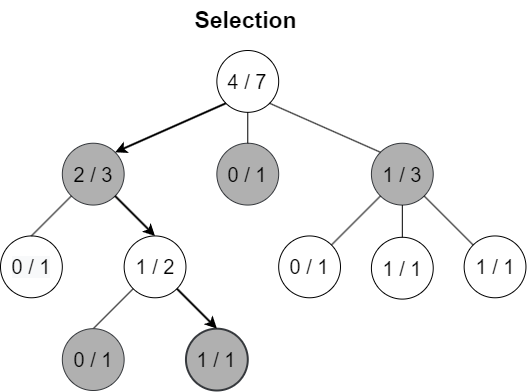
\includegraphics[width=.8\linewidth]{figures/MCTS Selection}
  \caption{Selection step}
  \label{fig:MCTS Selection}
\end{subfigure}%
\begin{subfigure}{.5\textwidth}
  \centering
  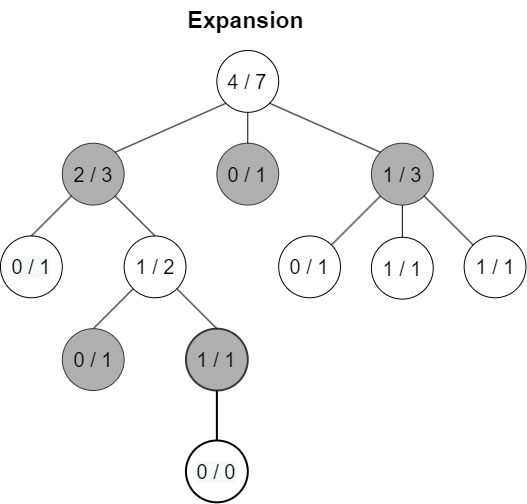
\includegraphics[width=.8\linewidth]{figures/MCTS Expansion}
  \caption{Expansion step}
  \label{fig:MCTS Expansion}
\end{subfigure}
\begin{subfigure}{.5\textwidth}
  \centering
  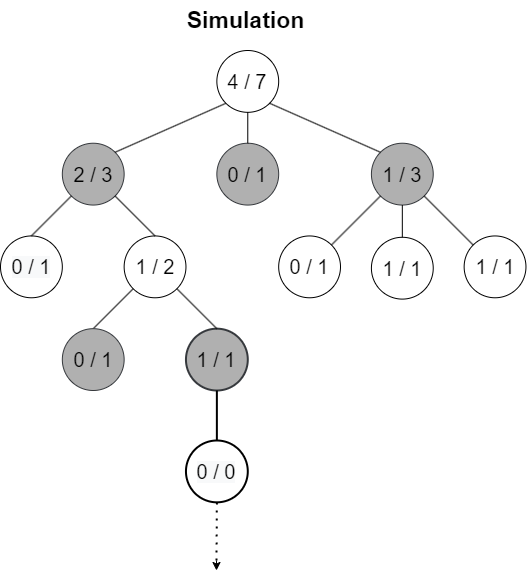
\includegraphics[width=.8\linewidth]{figures/MCTS Simulation}
  \caption{Simulation step}
  \label{fig:MCTS Simulation}
\end{subfigure}%
\begin{subfigure}{.5\textwidth}
  \centering
  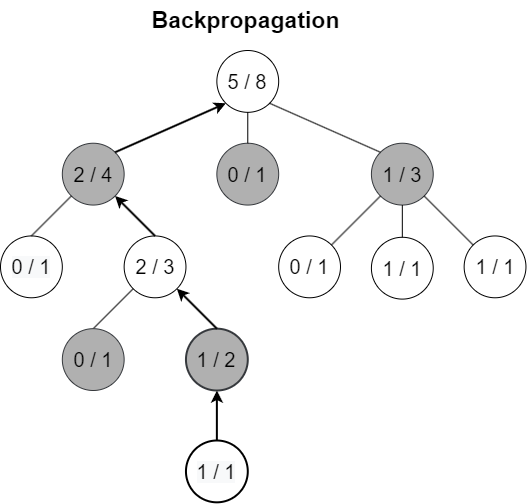
\includegraphics[width=.8\linewidth]{figures/MCTS Backpropagation}
  \caption{Backpropagation step}
  \label{fig:MCTS Backpropagation}
\end{subfigure}
\caption{A graph showing the steps of a Monte-Carlo Tree Search}
\label{fig:MCTS}
\end{figure}

If the leaf node does not terminate the game, it will create the next step with more child nodes throughout the tree, and if this simulated child node gives optimistic result probabilities it will update and back-propagate up the tree towards the root.
At its core, the \ac{MCTS} chooses the optimal move from the current state of a game's tree with the help of reinforcement learning.
Using this system, \citet{chen2018art} were able to achieve a win-rate of up to 88.0\% versus a standard association rule draft recommendation system used in studies such as \citet{hanke2017moba}. \\

Recently, \citet{shen2022deep} initiated studies into the champion recommendation using a mix of \ac{NLP} techniques and Bidirectional long-short term memory models.
They found that their proposed recommendation mechanisms were effective in both the coverage of champions and user satisfaction
Whilst this paper reiterated the fact that the champion selection phase can be predicted, it gives a unique perspective of adding a level of subjectivity to model by using user feedback and offers a wider-coverage of champions who are deemed less popular picks.
But this lack of objective measure gives it no quantifiable metric onto which this study can extract valuable information from. \\

These examples of predictive analytics for video games all employed machine learning strategies from Random Forest to \ac{RNN}s, and show that all are applicable to this task.
Demonstrated by many of these papers, the Random Forest performed particularly well with high predictive accuracy when applied to League of Legends or other similar games.
This leads to the conclusion that a decision tree based algorithm such as the Random Forest algorithm will likely be the best performing technique, with less overall evidence to support more linear methods such as Logistic Regression.

\section{Esports Betting}\label{sec:Esports Betting}
As esports has grown, so has the ability of bookmakers to capitalise on a new developing market and create revenue.
According to~\citet{absolute2022esportsbet}, the global esports betting market has been estimated to be worth up to \$10 Billion in 2021, and is forecasted to double by the year 2028 with a compound annual growth rate of 13.1\%.
A new focus of esports has grown throughout traditional bookmakers, with an increasingly larger number of esports titles to bet on and some bookmakers even sponsoring some events~\citep{esportsinsider2019}.
With the large variety of titles comes the challenge of creating odds that are representative of the outcomes that will occur.
There are numerous studies showing how gambling markets in most traditional sports can change how a given team is evaluated, often with regard to sentiment bias~\citep{feddersen2018sentiment, na2019not}.
This means that odds-makers must create predictive models that can accurately replicate the true likelihood of match outcome in order to ensure money is continually being made.
According to the efficient-market hypothesis, sport bets should be subject to all available information that may be publicly available and this information will be reflected in the odds themselves\citep{even1992testing}.
The betting market is therefore thought of as a fair and efficient market in which match outcomes can be accurately predicted.\\

Betting within esports has taken on many forms.
Money line bets and proposition bets are the most common types of bets.
Money line bets are bets that are placed on the outcome of a specific match, with payouts based on the odds that are created by the odds-makers using their internal prediction models.
Proposition bets are bets made based on whether a specific event will take place within the game itself while the match is ongoing.
A common proposition bet is whether a team would achieve the first kill of the game - commonly referred to as First Blood.
All these types of bets require highly calculated odds ensuring the bookmakers will make money.
With esports betting being in its early form, there are no regulatory structures put in place to effectively to keep match integrity in place similar to those found within most sports~\citep{dos2017q}.
This lack of match integrity causes potential match-fixing scandals which threatens the competitive integrity of both the league and the gambling market, as well as ruining games for spectators alike.
Whilst studies such as~\citet{abarbanel2019esports} claim that esports spectators aren't deeply concerned about potential match-fixing, with most spectators being willing to forgive infractions that have occurred previously.
Cases of match-fixing have already been investigated, with a Chinese player- `Bo' being suspended after being coerced into match-fixing in the Chinese academy leagues, subsequently causing a league-wide large-scale investigation~\citep{heath2021matchfixing}.
This caused a call for harsher punishments and stricter measures to ensure infractions like these would become highly disincentivised, however no regulatory structures apart from the league's punishment systems currently exist.

\section{Summary}\label{sec:Summary}
This chapter provided an overview of key literature in predictive analytics and its relation to both sports and esports.
Starting with a background on predictive analytics in sports, with the various uses scholars have modelled with and how their success can be replicated in the esports space.
This was followed with studies showing how these predictive analytics can be applied to various esport titles.
The various machine learning techniques that have been used previously were explained such as the Monte-Carlo Tree Search and the Random Forest classifier, with an exploration into how different machine learning techniques differ with results.
The betting industry was then explored, showing its relation to the world of esports and how they use prediction modelling for their business.
With the information gained throughout this literature review, the following research questions and research aims have been created:

\begin{quote}  \emph{Research Question 1: To what extent does the prediction accuracy of a League of Legends esports match outcome model increase through game time and why?} \end{quote}

\begin{quote}  \emph{Research Question 2: How strongly afflicted are League of Legends esports prediction models with multicollinearity issues and why?} \end{quote}

\begin{quote}  \emph{Research Question 3: How does the prediction accuracy of a League of Legends esports match outcome model vary based on the machine learning technique used?} \end{quote}

\begin{quote}  \emph{Research Aim 1: To assess the change in prediction accuracy of a League of Legends esports match through the progression of the match.} \end{quote}

\begin{quote}  \emph{Research Aim 2: To explore how the issue of multicollinearity in a League of Legends outcome model affects the prediction accuracy.} \end{quote}

\begin{quote}  \emph{Research Aim 3: To understand how the machine learning technique used in a League of Legends esports match outcome model can change its performance?.} \end{quote}